\section{UX - User Experience and Interface Design}

This Section describes the User Experience, meaning all the webpages that a customer will be able to reach and all the functionalities he will have access to.
\newline
We used a Class Diagram with three stereotypes:
\begin {itemize}
\item \textit{Screen $($yellow$)$:} represents regular webpages, like the HomePages.
\item \textit{Input Form $($blue$)$:} represents input fields, like the standard email-password form used to log in.
\item \textit{Regular Classes $($green$)$:} represents the Classes that are present in the regular Class Diagram.
\end {itemize} 
\hfill
\hfill

We divided our UX Diagram in three parts, in order to better highlight the connections between specified pages which have related functionalities:
\begin{enumerate}
\item \textbf{Log In, Sign Up and Data Editing}\\
	This UX Diagram shows the pages and the functions related to the management of the Customer data, like Log In, Sign Up and data modification
\item \textbf{Taxi Calls}\\
	Here all the connections between the pages used to call a taxi in all the possible ways are explained. 
	In the Booked Ride case the possibility to modify the reservation data is also shown.
\item \textbf{Driver's Pages}\\ 
	The last Diagram shows the pages created for the Driver's use via the app. 
	This includes functionalities like the status management and the job acceptance.
	
\end{enumerate}
\newpage

\subsection{Log In, Sign Up and Data Editing}
As shown in the diagram below, when someone opens either the website or the app he gets to the Guest's HomePage. Here he can call a taxi with the Instant Call function or fill the Input Form to Log In, in order to have access to the User's functions. Also a Guest that hasn't registered before can click on the \textit{Sign Up} button that will take him to the dedicated webpage, where he can fill in the fields and register.\\
Users can also modify their data getting into the User Profile webpage and modifying an Input Form similar to the Sign Up one. \\
Lastly, Taxi Drivers $($only via app$)$ can perform their special Log In to get to the Driver's special HomePage. 

	\begin{figure}[h!]
		\centering
		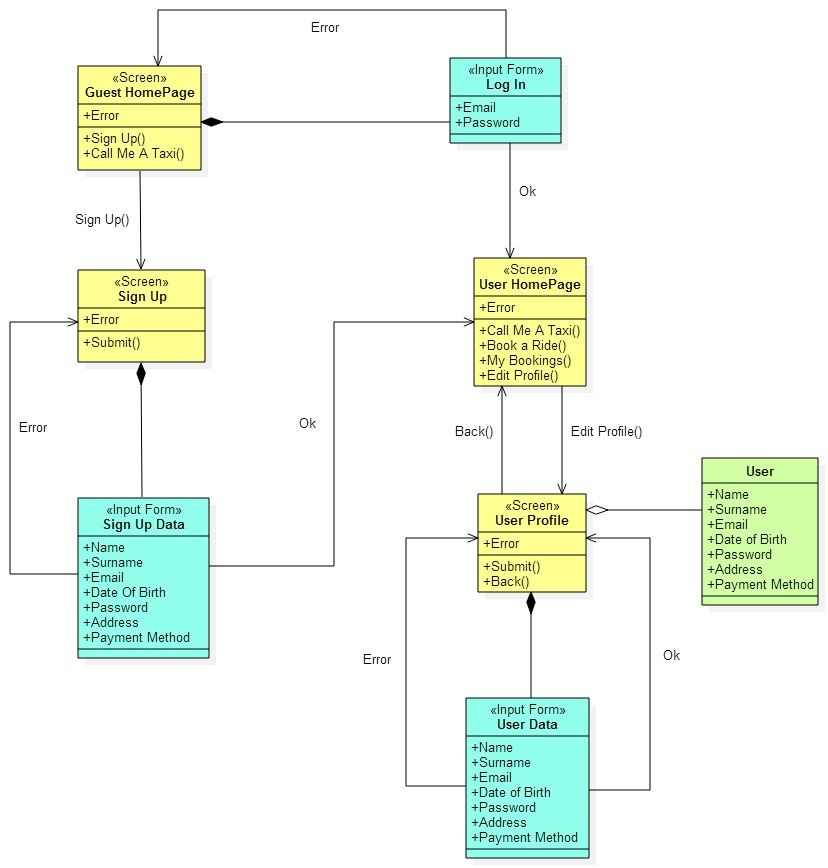
\includegraphics[height=0.65\textheight]{UXDiagrams/UXProfile.jpg}
	\end{figure}
	
\newpage
\subsection{Taxi Calls}
As described in the RASD, the Instant Call is a functionality that is granted to both Guests and Users; for this reason, the \textit{Call Me a Taxi} button is present in both the HomePages. \\
In the Instant Call page the Customer can fill an Input Form to specify his location and the payment method.\\
On the other hand the Booking and sharing functions are User exclusive, so the dedicated button is only in his HomePage. This button opens a page with an Input Form used to specify all the data about the requested ride and lets a user eventually enable the Sharing option.\\
A User also has the possibility to visualize his past rides and see the data of the booked ones. By clicking the \textit{Status} button a page with the current state of a ride and will be given the possibility of cancel or modify it $($if it's not locked$)$ will be shown.

\begin{figure}[h!]
\centering
		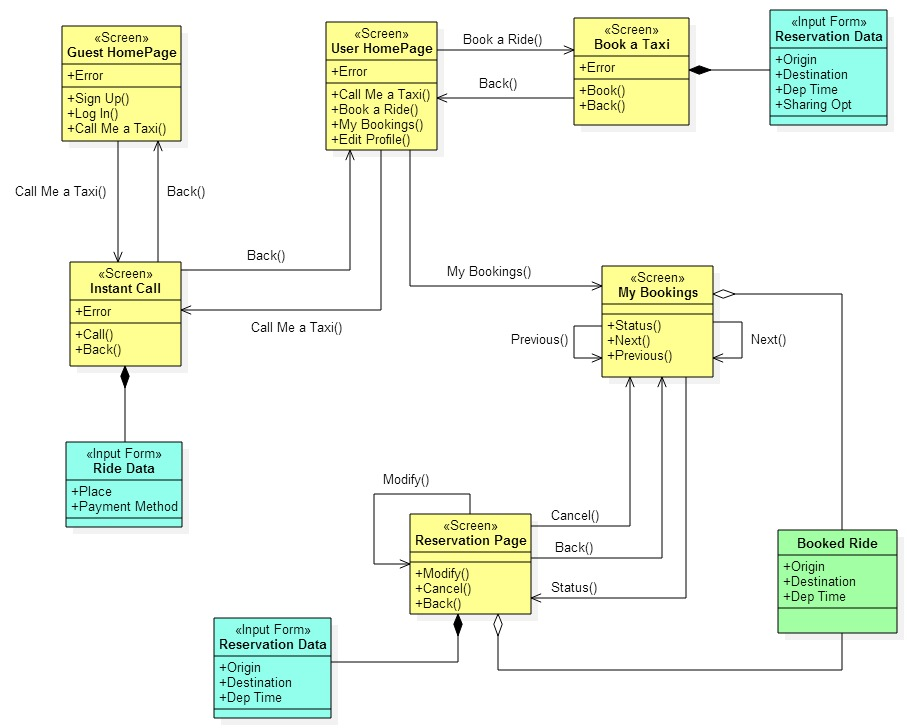
\includegraphics[width=1\textwidth]{UXDiagrams/UXBooking.jpg}
	\end{figure}

\newpage
\subsection{Driver's Pages}
The Driver's part of the UX Diagram is much simpler than the others because the Driver is supposed access the system only via mobile. Most of the functionalities are accessible from the main page, like the one concerning the management of the working status. \\
The only other page viewable is the Ride Page, shown when a notification of a new possibile job is recieved. In this page the Driver can see the Ride's data and decide if accept it or not.
\\
\begin{figure}[h!]
		\centering
		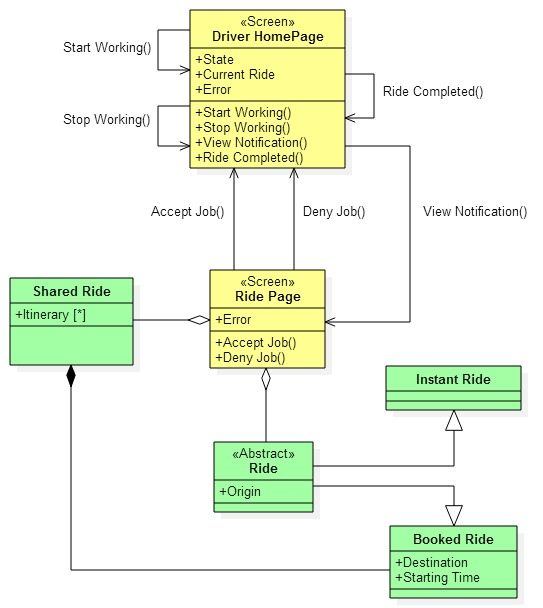
\includegraphics[height=0.7\textheight]{UXDiagrams/UXDriver.jpg}
	\end{figure}